\chapter{One-to-many Relationships}
\label{chapter:representing-relationships}

One-to-many relationships
%such as those in an entity-relationship model,
are typically implemented in Java using the standard library collection classes.
Each object maintains a collection of the objects related to
it along a given relationship. Since one-to-many relationships are such an
important part of most data models, it is not uncommon for Java applications to
need hundreds of thousands, or even millions, of collections.
Therefore, simple decisions, like which collection class to choose,
when to create collections, and how to initialize them,
can make a big difference on memory cost.
This chapter shows how to lower memory costs when implementing
relationships with collections.
 
 \section{Choosing the Right Collection for the Task}
 \label{section:choosing-collection}

The standard Java collection classes vary widely in terms of how much memory they use.
Not surprisingly, the more functionality a collection provides, the more
memory it consumes. Collections range from simple, highly efficient
\class{ArrayList}s to very complex
\class{ConcurrentHashMap}s, which offer sophisticated concurrent access
control at an extremely high price. 
Using overly general collections, that provide more functionality than
really needed, is a common pattern leading to excessive memory bloat.
This section looks at what to consider when choosing a collection to
represent a relationship. 

Using collections for relationships often results in many small or
empty collections.  That's because for a given relationship there are
usually lots of objects that are related to either just a few other
objects or to none at all.
When there are lots of collections with only a few entries, you need to ask  whether
the functionality of the collection you choose is worth the memory cost of that
functionality\footnote{We'll use the shorthand
\emph{relationship} to mean a one-to-many relationship, unless otherwise noted. 
We'll also use \emph{small collection} to mean a very small collection, where
the number of elements is roughly in the single digits.}

To make this discussion more concrete, let's return to the product and supplier example 
from section~\ref{sec:rarely-used}, and change it a little
 bit. Instead of only one alternate supplier, a product now may have multiple
 alternate suppliers, and each product stores a reference to a collection of alternate suppliers. An obvious choice is
 to store the alternate suppliers in a \class{HashSet}:
 \begin{shortlisting} 
class Product {
	String sku;
	String name;
	.. 
	HashSet<Supplier> alternateSuppliers;
}

class Supplier {
	String supplierName;
	String supplierAddress;
	String sku;
}
\end{shortlisting}


Suppose there are 100,000 products that each have four alternate suppliers on
average. Figure~\ref{fig:product-hashset} shows an entity-collection diagram for
the relationship between products and alternate suppliers.
 \begin{figure}
  \centering
 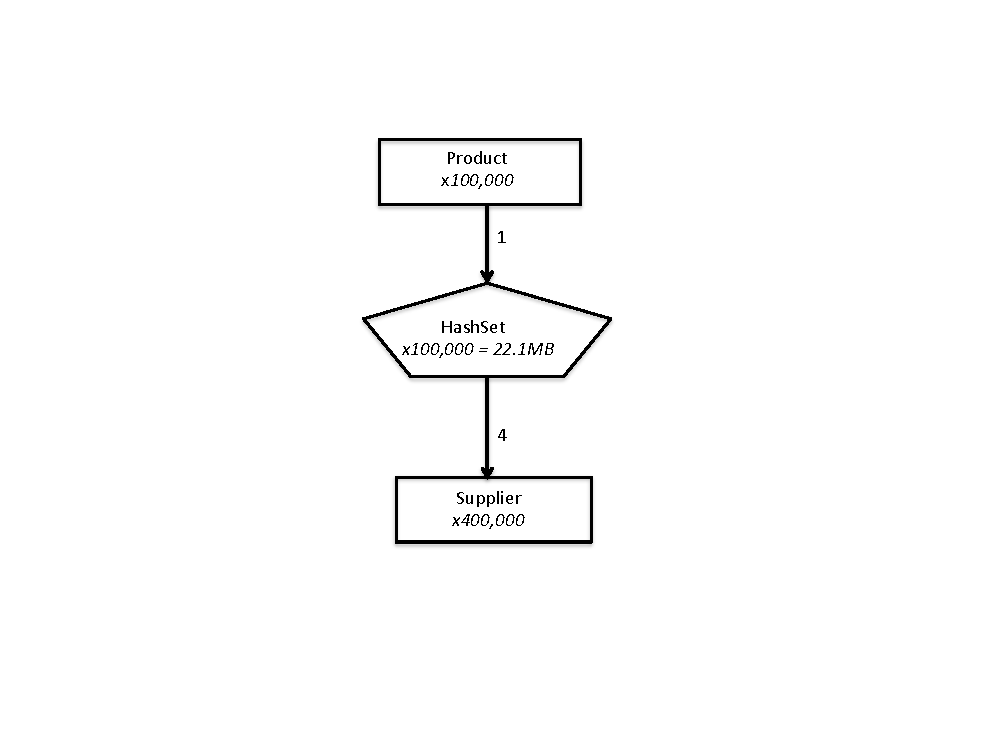
\includegraphics[width=.80\textwidth]{part1/Figures/collections/product-hashset.pdf}
 \caption{A relationship between products and alternate suppliers.
  Stored as one
  \class{HashSet} of alternate \class{Suppliers} per \class{Product}.}
  \label{fig:product-hashset}
\end{figure}


Using a \class{HashSet} for alternate suppliers turns out to be a
very costly decision. The alternate suppliers are represented by 100,000
very small \class{HashSet}s, each consuming 232 bytes, for a total cost of 22.1MB. 
This cost is all overhead.
It's hard to think of a good reason why such a heavy-weight collection should ever be used
 for storing just a few entries, and yet, this pattern is very, very common. For
 small sets, \class{ArrayList} is almost always a better choice. \class{HashSet}
 does maintain uniqueness, but enforcing uniqueness
in the data model is not always needed. Many applications
 perform this check in their loading code. If it is
important to guarantee uniqueness in the data model, it can be enforced for an
\class{ArrayList} with  little extra checking code, and usually without significant performance
 loss when sets are small.  Figure~\ref{fig:product-arraylist} shows improved memory usage with
 \class{ArrayList}. Each \class{ArrayList} incurs 80 bytes of overhead, approximately a third the size of
 a \class{HashSet}.
 \begin{figure}
  \centering
 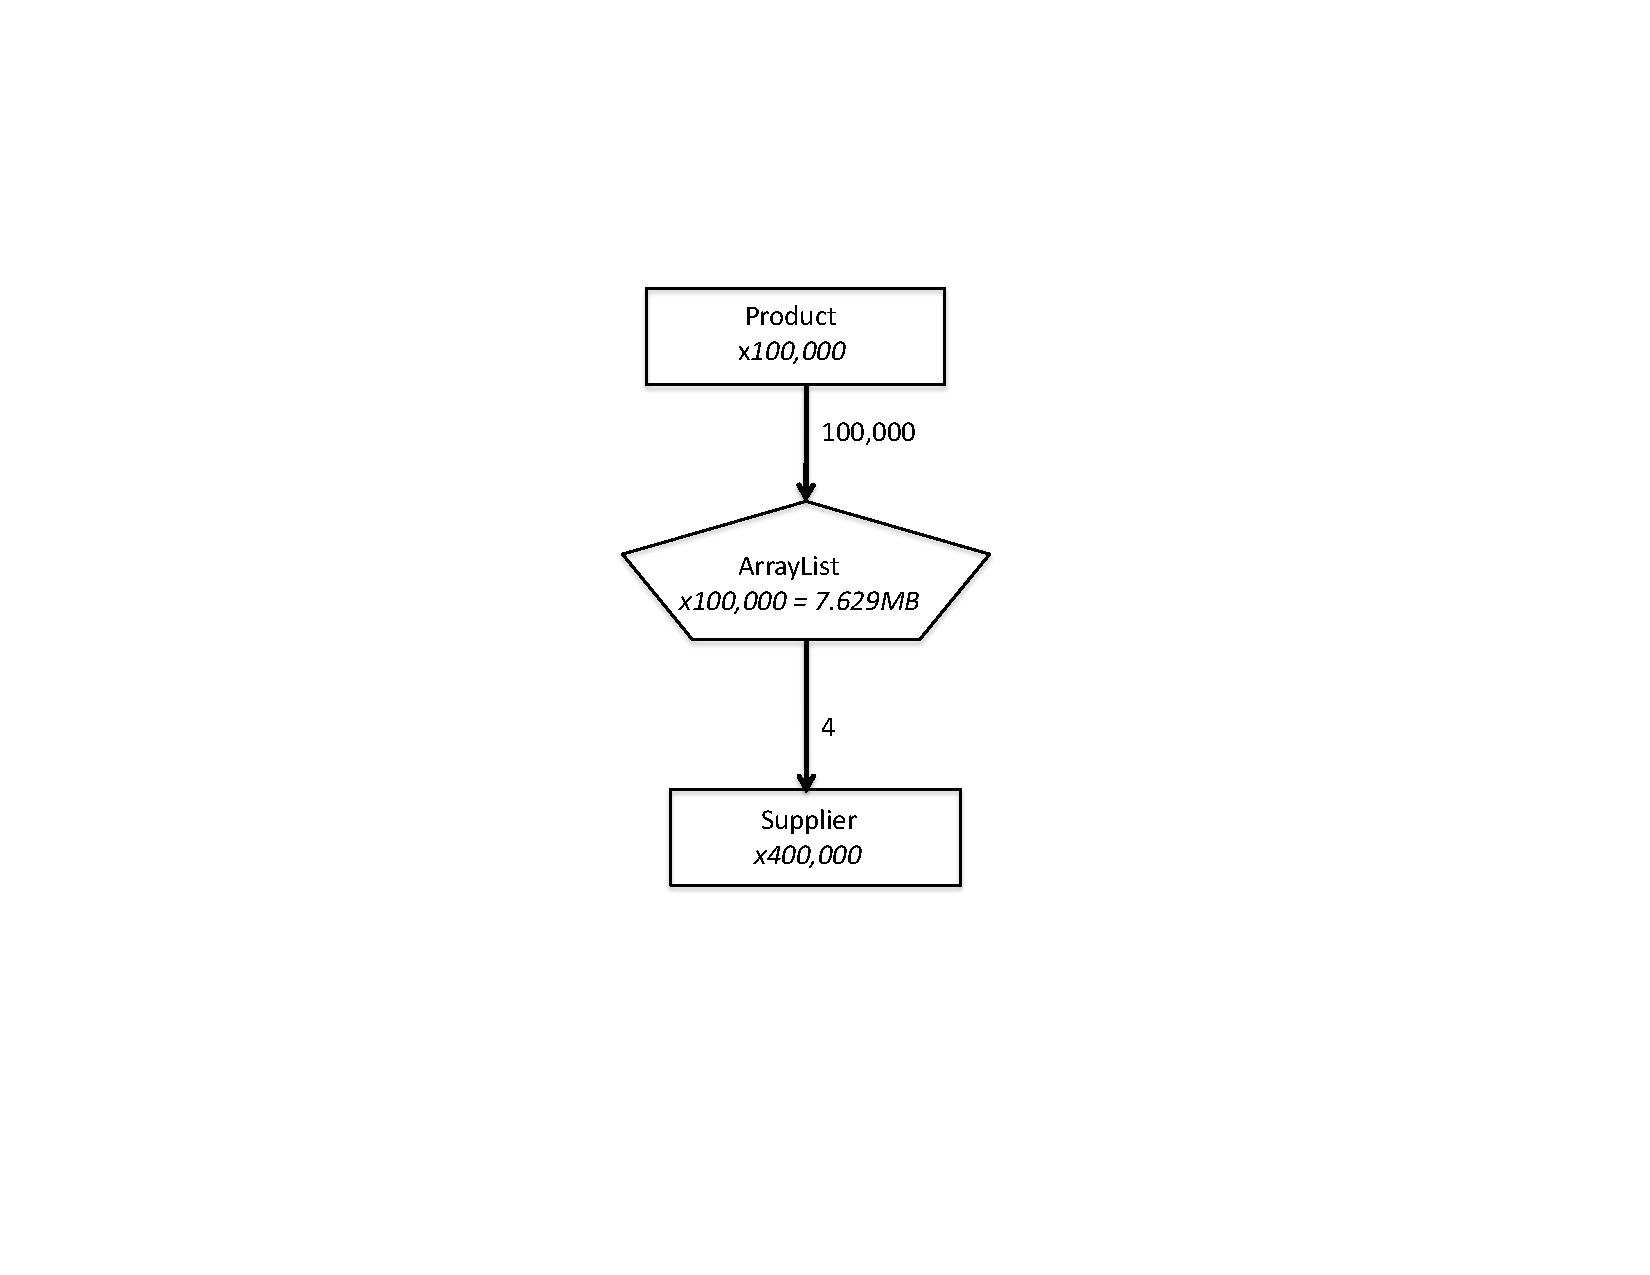
\includegraphics[width=.80\textwidth]{part1/Figures/collections/product-arraylist.pdf}
 \caption{A relationship between 100,000 products and alternate suppliers,
 where the alternate \class{Supplier}s associated with each
 \class{Product} are stored in an \class{ArrayList}.}
  \label{fig:product-arraylist}
\end{figure}
This simple change saves 14.5MB. 


\section{Inside Small Collections}
\label{sec:collectioncost}
Let's look inside a \class{HashSet} to see why it is so much bigger than an
\class{ArrayList}.
The structure of a \class{HashSet} is shown in
Figure~\ref{fig:inside-hashset}. All
collections have a similar basic structure: a wrapper
which remains stable, and an internal structure that changes as entries are
added and removed.

The standard library designers implemented
\class{HashSet} by delegating its work to a degenerate \class{HashMap},
that is, one with keys but no values.
The \class{HashSet} object is therefore just a wrapper, and it points to a
\class{HashMap} wrapper. All collections have
wrapper objects, but a \class{HashSet} has two of them. 
%Together they incur a fixed cost of 56 bytes.

\class{HashMap} itself uses a \emph{chaining}
design. Its internal structure is an array of hash buckets, with initial size of
16 by default.  Each bucket is a linked
list of \class{HashMap\$Entry} objects. Each entry object
points to an element of the user's data, in other words, to a key and value.

 \begin{figure}
  \centering
 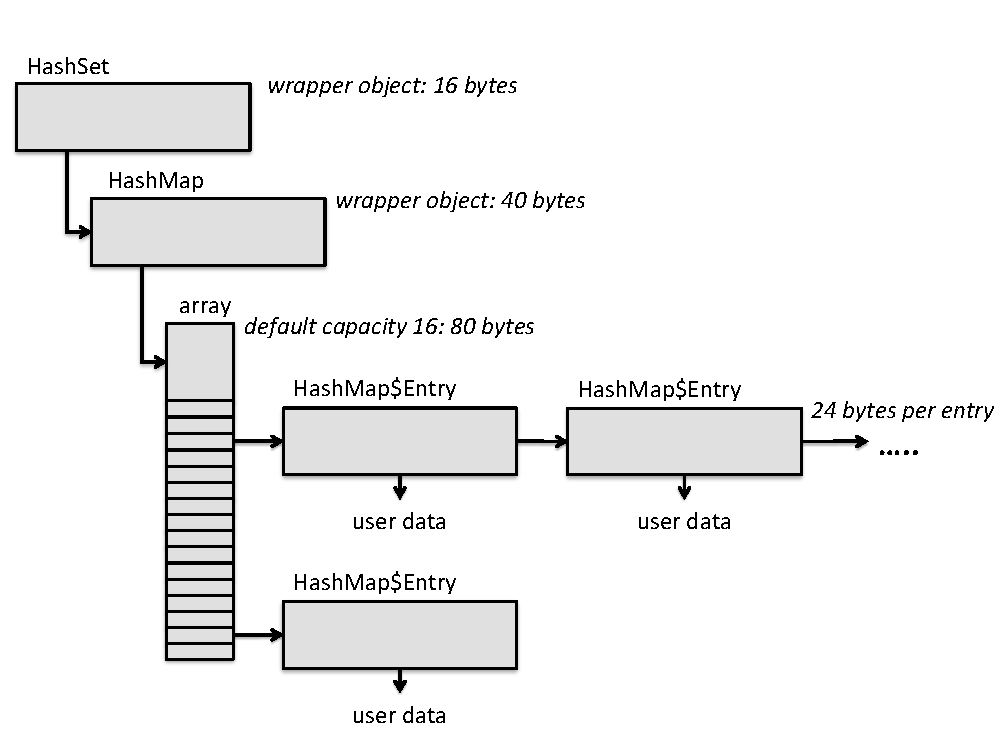
\includegraphics[width=.80\textwidth]{part1/Figures/collections/inside-hashset.pdf}
  \caption{A look inside a \class{HashSet}. Shown with 3
  entries.}
  \label{fig:inside-hashset}
\end{figure}

In contrast, \class{ArrayList} is a simpler structure, as shown in
Figure~\ref{fig:inside-arraylist}. It's an expandable array,
consisting of a wrapper object and an array.  The array points directly to the
user data. The array has an initial size of 10 by default.  As a result of its
simpler design \class{ArrayList} has a smaller fixed cost and a smaller
variable cost than \class{HashSet}.

The fixed cost is the memory needed before any entries are added.
For a \class{HashSet} this is the two wrapper objects, at 56 bytes, plus
the array's \jre overhead and 16 slots,
80 bytes, bringing the total to 136 bytes. We count the array's empty slots as a
fixed cost, since they are allocated right from the start
\footnote{\class{HashSet} has another fixed cost that occurs in a
common usage scenario.  If you iterate over the contents of the set, a 16-byte
\class{HashMap\$KeySet} object will be created and retained for the lifetime of
the set. We don't include this in any of our numbers.}.
The fixed cost of a default-sized \class{ArrayList} is considerably
lower, a total of 80 bytes. That includes its wrapper object and default
10-element array. Fixed costs matter most in
small collections; as a collection grows they become less significant.

\footnote{As a collection grows beyond its initial size, it makes more sense to
treat excess capacity as a variable cost, as we'll discuss in the next chapter.
This is because growth policies typically allocate excess capacity
in proportion to the size of the collection}.

A \class{HashMap\$Entry} is maintained for
each entry, at 24 bytes each. This is the collection's variable
cost, that is, the incremental cost of storing an
entry

The variable cost of a \class{HashSet} is 24 bytes. The variable cost of a small
\class{ArrayList} can be considered 0, since by default the array has been
allocated with 10 extra slots. Lower variable
cost means that \class{ArrayList} scales much better than \class{HashSet}. 
So \class{ArrayList} is better both for small and large sets.
 \begin{figure}
  \centering
 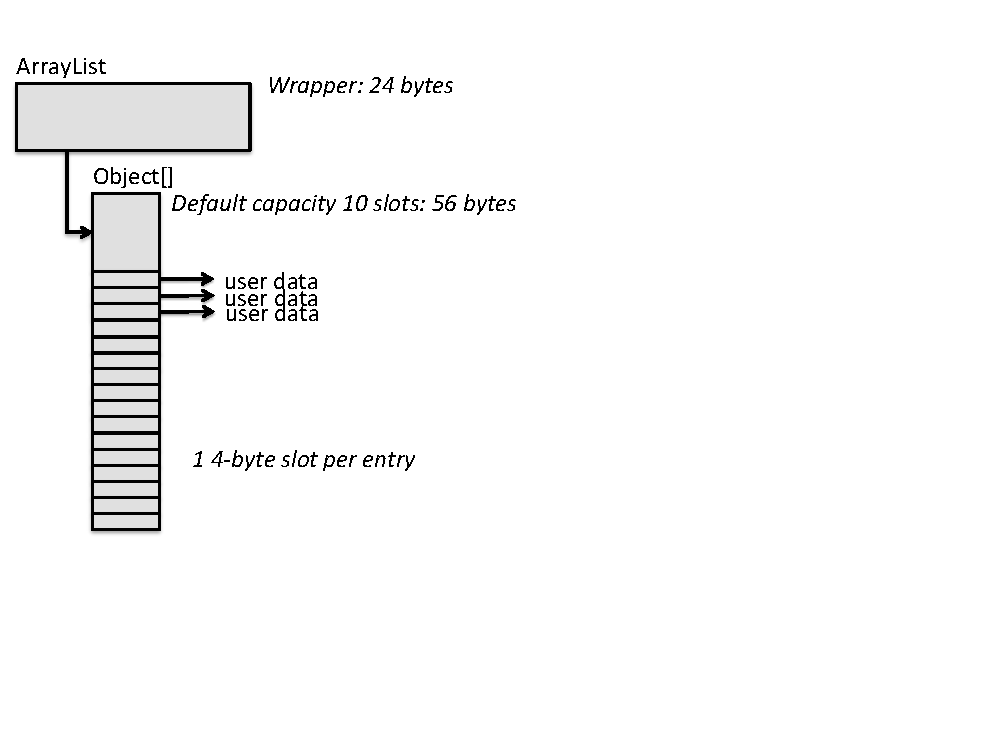
\includegraphics[width=.80\textwidth]{part1/Figures/collections/inside-arraylist.pdf}
 \caption{Inside an \class{ArrayList}. Shown with three
 entries and default capacity. \class{ArrayList} has a relatively low
 fixed overhead, and is scalable.}
  \label{fig:inside-arraylist}
\end{figure}
 

Table~\ref{tab:small-collections-default} shows the memory costs of four common
collection classes, \class{ArrayList}, \class{LinkedList}, \class{HashMap}, and
\class{HashSet}.
This table shows the default size when the collection is just allocated without
entries, and any additional entry cost. These costs have
been calculated based on the Sun JVM, using the techniques described in Chapter~\ref{chapter:delegation}. 
The various other Java standard
library implementations in circulation have costs
similar to these. You can calculate them using the same methodology.


\begin{table}
\centering
 		\begin{tabular}{l||r||r||rrl}
 		\toprule
	 	 Collection & \makebox{with 1 entry} & \makebox{with 4 entries} &
	 	 \multicolumn{3}{c}{with n entries}\\
	 	 & & & Fixed & Variable & Range \\
	 	 \midrule
	 	ArrayList & 80 & 80 & 80 & 0 & 0 .. 10 \\
 		HashMap & 144 & 216 & 120 & 24 & 0 .. 11 \\
 		HashSet & 160 & 232 & 136 & 24 & 0 .. 11 \\
 		LinkedList & 72 & 144 & 48 & 24 & any n \\
	 	\bottomrule
	 	\end{tabular}
	 	
	\caption{Costs of some common collections when they
	contain very few entries and are allocated with default capacity. Variable
	cost is the cost per entry, above the fixed cost of the collection. Costs apply only within the specified range.}
	\label{tab:small-collections-default}
\end{table}
\begin{table}
\centering
 		\begin{tabular}{l||r||r||rrl}
 		\toprule
	 	 Collection & \makebox{with 1 entry} & \makebox{with 4 entries} &
	 	 \multicolumn{3}{c}{with n entries}\\
	 	 & & & Fixed & Variable & Range \\
	 	 \midrule
	 	ArrayList & 48 & 56 & 40 & (n/2)*8 & any n \\
 		HashMap & 112 &     & 64 & 24 & 0 .. 1 \\
 		        &     & 184 & 88 & 24 & 2 .. 5 \\
 		HashSet & 128 &     & 80 & 24 & 0 .. 5 \\
		        &     & 200 & 104 & 24 & 2 .. 5 \\
	 	\bottomrule
 	 	\end{tabular}
	\caption{Costs of some common collection classes when capacity is set to the
	minimum to accomodate the number of entries shown.}
	\label{tab:small-collections-minimum}
\end{table}

The fact that \class{HashSet} delegates to \class{HashMap} inflates its fixed
cost in two ways: the cost of the extra wrapper object, and the cost of fields
in the \class{HashMap} that aren't needed when it's used as a set. 
Note that since the \class{HashMap\$Entry} class is designed for
a \class{HashMap}, its value field is not used.

Some of its extra cost is because of additional functionality,
such as providing uniqueness checking and entry removal in constant time.
\class{HashSet} is also optimized for performance, and sacrifices memory 
under the assumption that \class{HashSet}s will contain a large number of
elements. Additionally, \class{HashSet} delegates its work to a
degenerate \class{HashMap}, that is, one with keys but no values. This decision,
to reuse the more general \class{HashMap} code, adds to the memory
cost. Other extra costs are due to unavoidable Java overhead.

Our guess is that the
collection class developers would be surprised by the relationship usage pattern
that results in hundreds of thousands of small \class{HashSets}. Why bother
implementing expandable structures and clever hashing algorithms for only a few entries?
This mismatch between collection implementation and usage is 
a leading cause of memory bloat. The overhead cost of a \class{HashSet} is
remarkably high. Creating many small collections multiplies this basic infrastructure
cost, which is all overhead, filling the heap. 
 

\section{Properly Sizing Collections}
\label{sec:proper-size}

Many collection classes, such as \class{ArrayList}, \class{HashMap} and
\class{HashSet}, use arrays in their implementations. When the array becomes
full, a larger array is allocated and the contents are copied into the new array.
Since allocation and copying can be expensive, these arrays are
allocated with extra capacity, to avoid paying these growth costs too
often. 
%This is why
By default, the initial capacity of an \class{ArrayList} is 10, and the capacity
increases by 50\% whenever the array is reallocated.
The default capacity of a \class{HashMap} or \class{HashSet}
starts at 16, and grows by a factor of 2 when the collection becomes 75\% full.

These policies trade space
for time, on the assumption that collections always grow.
However, many applications have relationships with
hundreds of thousands of collections that do not grow once the data has
been loaded. Most may never contain more than a few elements. 
In these cases, the empty array slots can add up to a
significant bloat problem, with nothing gained in performance. 
The same holds true for larger collections that stop growing. 
%,unless you take explicit action.

Fortunately, it is often possible to right-size collections at creation
time, by specifying an initial capacity. For example, if you know that an
\class{ArrayList} has a maximum size of $x$, which is less than the default
size, then you can set its initial capacity to $x$ when calling its constructor. On the
other hand, the standard collections do not give you much control over their
growth policies. So if you are wrong and the \class{ArrayList} grows bigger than
$x$, extra capacity will be allocated, which may be worse than just taking the
default. 
 
For an \class{ArrayList}, another approach is to call its \code{trimToSize}
method, which shrinks the array by eliminating the extra growth space. 
Since trimming reallocates and copies the array, it is expensive to call
\code{trimToSize} while a collection is still growing. Trimming is
appropriate after a collection is fully populated. In 
applications where the data has a build phase followed by a use phase,
the \class{ArrayList}s can be trimmed between these two phases.
%so that the cost of reallocation and copying is paid only once.
 
Returning to the example of the relationship between products and alternate
suppliers, the \class{ArrayList}s in Figure~\ref{fig:product-arraylist} have
been initialized with default capacity. If we assume that the the relationship
is built in one phase and used in another phase, then it is possible to trim the
\class{ArrayList}s after the first phase. This should save quite a bit of
space, since there are 100,000 \class{ArrayList}s with four entries on
average. In fact, trimming these
\class{ArrayList}s saves 2.3MB, or another 30\%, as shown in
Figure~\ref{fig:trimmed-product}. 

\begin{figure}
  \centering
 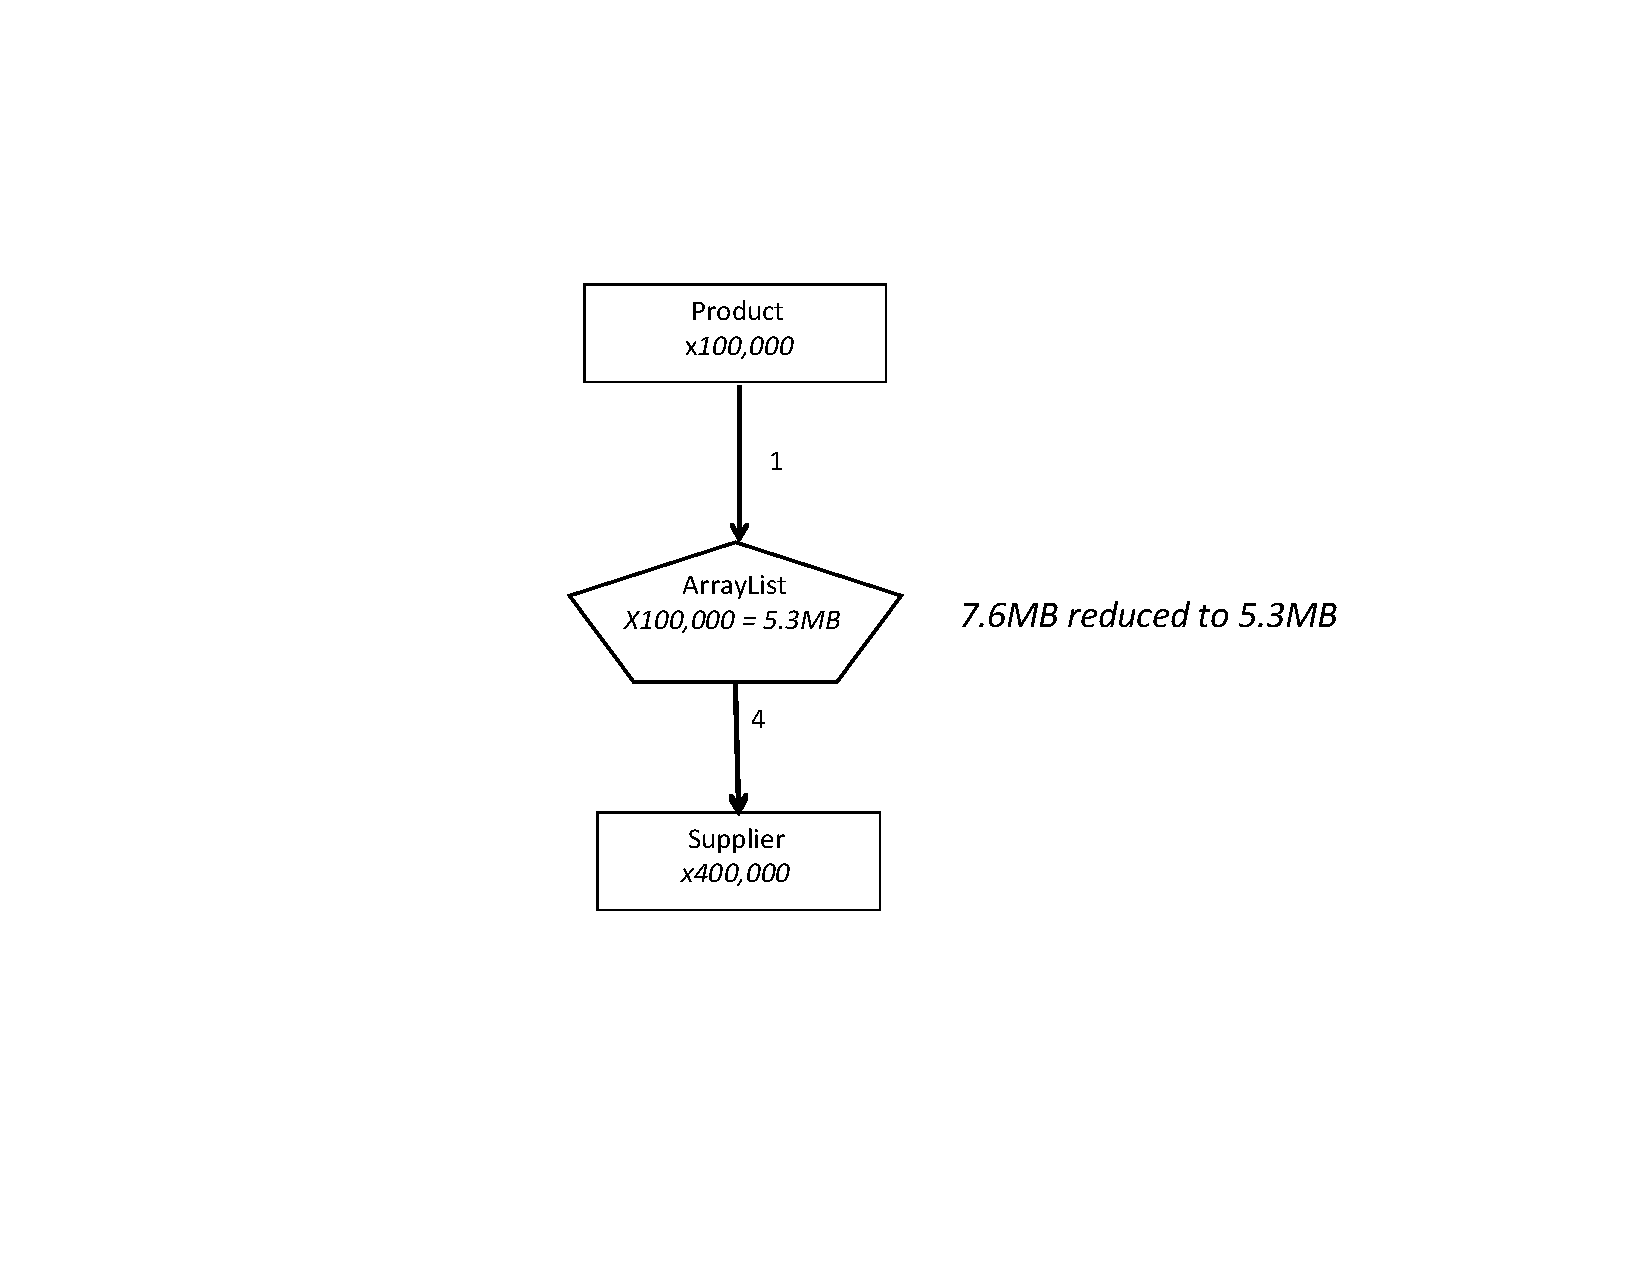
\includegraphics[width=.80\textwidth]{part1/Figures/collections/trimmed-product.pdf}
 \caption{The relationship between \class{Product}s and \class{Supplier}s after
 all of the
 \class{ArrayLists} have been trimmed by calling the \code{trimToSize} method.}
  \label{fig:trimmed-product}
\end{figure}
 
\class{HashSet}s and \class{HashMap}s do not have \code{trimToSize}
methods, but it is possible to set their initial capacity at construction time.
The initial capacity is the number of hash buckets, that is, the number of slots
in the array. It is automatically rounded up to the nearest power of
two. Hash-based collections always require some excess capacity to reduce the
likelihood of collisions. In addition, if the collection does grow and the
array needs to be reallocated, there will be the expense of
rehashing the entries. The load factor, by default .75, determines the
maximum number of elements in the collection relative to the size of the array,
before a larger array needs to be allocated. When setting the initial
capacity it's important to take the load factor into account, so that you leave enough headroom.

An \class{ArrayList}, \class{HashMap}, or \class{HashSet}
will not automatically reduce the size of its array when elements are removed,
or when the collection is cleared.

%However, before changing the initial capacity, you should
%ask yourself whether using a \class{HashSet} or \class{HashMap} is a
%wise decision in the first place. If you are going to end up with many
%collections with fewer than 16 elements, perhaps there is a more
% memory-efficient solution, like \class{ArrayList}.
  
%A \class{LinkedList} is another alternative for small collections, and are
%better than \class{ArrayLists} if the collections are changing a lot. The
%24 byte per-entry cost is larger, but there is no element array, and only one
%extra entry, which is a sentinal.

\section{Avoiding Empty Collections}

Maintaining a large number of empty collections is another common problem that
leads to memory bloat. Empty collection problems are generally caused by eager
initialization, that is, by allocating collections before they are actually
needed. You might think that eager initialization would not be a big
problem, since entries will be added eventually. However, it's common to
find large numbers of collections that remain empty throughout an execution.

Making matters worse, the standard collections
allocate their internal objects in an eager fashion. For example,
\class{ArrayList} allocates its internal array before any
entries are inserted, and \class{LinkedList} always allocates a sentinel
entry. As a result, every empty collection takes two or more objects, as shown
in \autoref{fig:inside-empty}.
This is true even if you allocate the collection with the minimum possible
capacity.
Therefore, the smallest empty collections are still quite large. For example,
a zero-capacity \class{ArrayList} requires 40 bytes.
\autoref{tab:empty-collection-costs} shows the sizes for some common collection classes
when empty. 

%a zero-sized \class{ArrayList}
%consumes 40 bytes, the smallest \class{HashMap} takes 64 bytes, and the
% smallest \class{HashSet} takes 80 bytes. Table 

%A quick look inside the empty collections show that they
%are not all that empty! 


 \begin{figure}
  \centering
 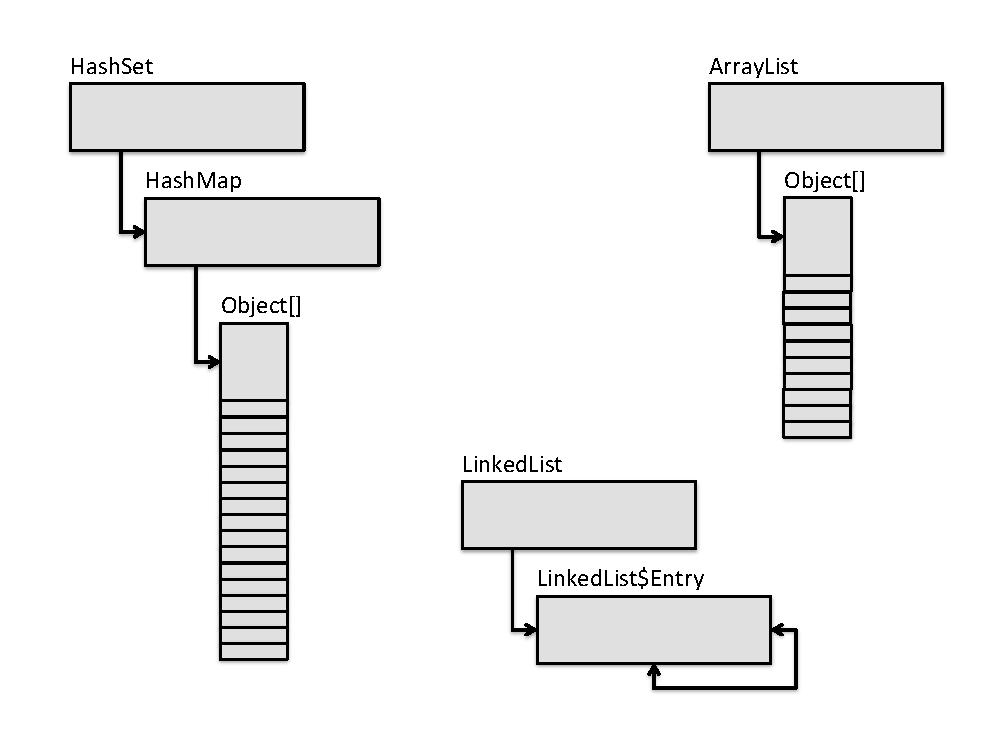
\includegraphics[width=.80\textwidth]{part1/Figures/collections/inside-empty.pdf}
  \caption{The internal structure of three empty collections. Each
  requires at least two objects, before any entries are added.}
  \label{fig:inside-empty}
\end{figure}

\begin{table}
\centering
 		\begin{tabular}{lcc}
 		\toprule
	 	 Collection & \multicolumn{2}{c}{Size in bytes} \\
	 	 & default capacity & minimum capacity \\
	 	 \midrule
	 	ArrayList & 80 & 40 \\
 		LinkedList & 48 & 48 \\
 		HashMap & 120 & 64 \\
 		HashSet & 136 & 80 \\
	 	\bottomrule
	 	\end{tabular}
	\caption{Size of empty collections, for some common
	collection classes.
	Empty collections require a lot of space, even when initialized to the smallest
	possible capacity.}
	\label{tab:empty-collection-costs}
\end{table}

\paragraph{Example} Suppose the relationship
in Figure~\ref{fig:trimmed-product} is initialized by the code:
%\begin{shortlisting}
%List<Product> products;
%int numProducts;
%..
%public void initAlternateSupplierRelationship() {
%	..
%	for (int i = 0; i < numProducts; i++) {
%    	Product product = products.get(i);
%		product.alternateSuppliers = 
%                           new ArrayList<Supplier>();
%    }
%}
%\end{shortlisting}

\begin{shortlisting} 
class Product {
	.. 
	ArrayList<Supplier> alternateSuppliers;
	..
	public Product() {
		..
		// Allocate the collection in advance
		alternateSuppliers = new ArrayList<Suppliers>();
		..
	}
}
\end{shortlisting}
Initially, each product allocates an empty \class{ArrayList} for alternate
suppliers, so there are 100,000 empty \class{ArrayLists} before any
\class{Supplier}s are inserted. As the alternate suppliers are populated, many
of these \class{ArrayLists} will become non-empty, but it is likely that a good
number of products have no alternate suppliers. If 25\% of the products have no
alternate suppliers, there will be 25,000 empty \class{ArrayLists}, which consume
about 1MB even after calling \code{trimToSize}.
Figure~\ref{fig:empty-array} shows the entity-collection
diagram after removing 25,000 empty alternate supplier \class{ArrayList}s.
The diagram now shows only 75,000 alternate supplier \class{ArrayList}s,
since there are no more empty \class{ArrayList}s. We therefore adjust the
average fanout in and out of \class{ArrayList} to .75 and 5.33, respectively.
\begin{figure}
  \centering
 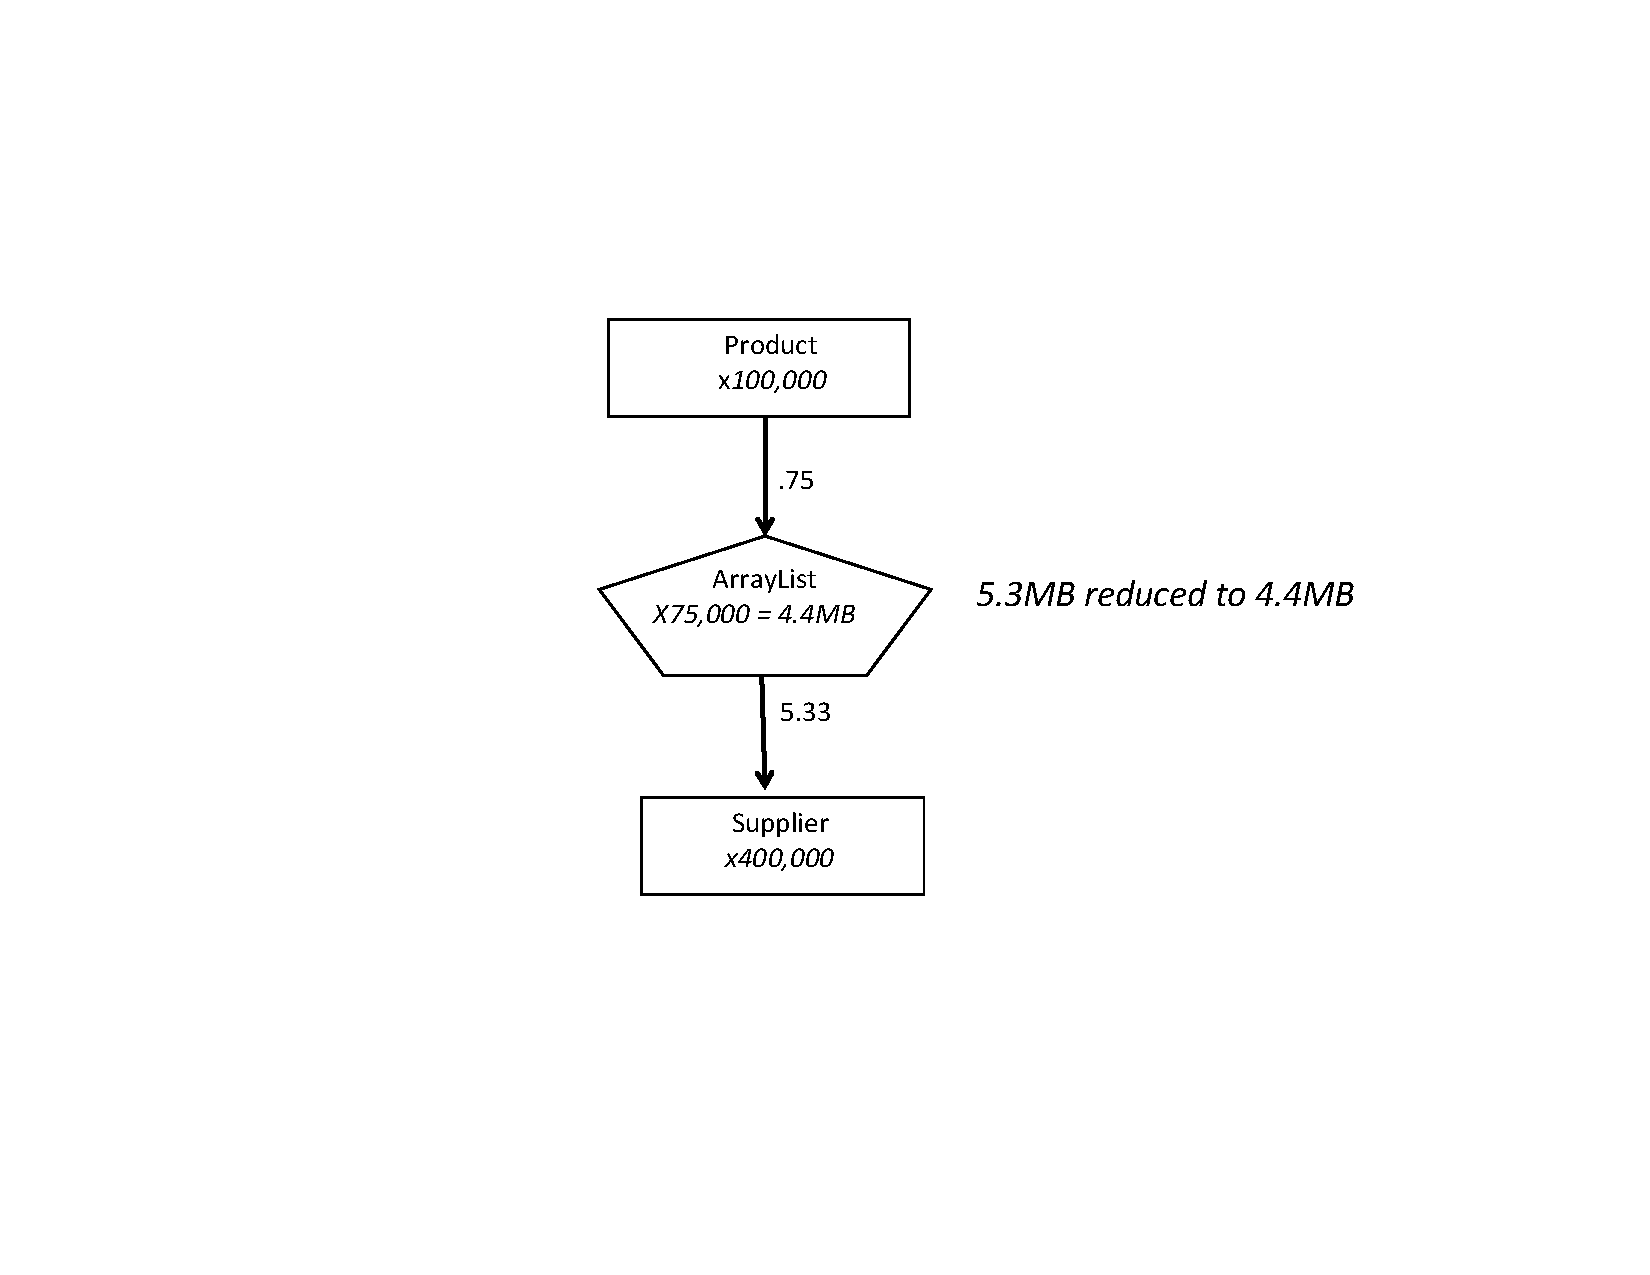
\includegraphics[width=.80\textwidth]{part1/Figures/collections/empty-product.pdf}
 \caption{The relationship between \class{Product}s and \class{Supplier}s,
  with no empty \class{ArrayLists}.}
  \label{fig:empty-array}
\end{figure}
 
 \paragraph{Lazy allocation} Delaying allocation is the way to
 avoid creating lots of empty collections.
 That is, instead of initializing all of the collections that you think you
 may need, allocate them on demand. 
 One approach is simply to leave collection fields null
 until needed. However, this requires extra checking code whenever you
 access these fields, to avoid \code{NullPointerException}s.
 
For many applications, the abstract
\class{Collections} class provides a better solution. You can initialize
collection fields to point to shared, immutable empty collections, using the
static methods \code{emptySet()}, \code{emptyList()}, and \code{emptyMap()}
\footnote{Static constants EMPTY\_SET, EMPTY\_LIST, and EMPTY\_MAP provide a similar capability,
without the type safety of generics.}.
The following code
maps all products to a single, immutable, empty list of suppliers, so that no
empty \class{ArrayLists} are created:

\begin{shortlisting}
class Product {
	.. 
	List<Supplier> alternateSuppliers;
	..
	public Product() {
		..
		// Initialize to a shared, static collection
		alternateSuppliers = new Collections.emptyList();
		..
	}
}
\end{shortlisting}

This initialization avoids the need to check whether an \class{ArrayList}
exists at every use. The size method, iterators, and other access functions
work as in any other collection.
However, you have to be careful not to let any references to these static empty
collections escape their immediate context. If you do give out a reference, 
then there is no way to update this reference once an actual collection is
allocated. Instead, you can provide access and update methods to the relationship,
so that the implementation remains hidden.
You will also need to code to interfaces, delaying the use of a concrete class
until a collections is actually allocated. In this example, \code{Product}
declares a \code{List} of suppliers, so that it can point to either the shared
empty list, or to an \class{ArrayList} once it's populated.
This is, of course, a good practice in general, so that the implementation can
be easily changed later.

If lazy allocation is not a good option for your application, then
right-sizing collections, at initialization time or after loading is
completed, will still make a difference for empty collections.

\section{Fixed Size Collections}

Java collections can grow to be
arbitrarily big, but this functionality comes at a cost.
Collections include wrapper objects, and 
may be sized with extra growth room. If
you know that the size of a collection is fixed, having the ability to expand
the collection is unnecessary, and it is better to choose a cheaper alternative.
In fact, often you can use a
simple Java array, and not use a collection at all.  

In our example, alternate suppliers are stored in an
 \class{ArrayList}, which inside is a
wrapper pointing to an array of \class{Suppliers}.  If we assume that
every product has at most four alternate suppliers, then  it isn't 
necessary to store these in an \class{ArrayList} --- a simple array will do.
Eliminating the \class{ArrayList} object removes 24 bytes per
product, but we have to add 4 bytes to each \class{Product} to store the number
of alternate suppliers. The total savings is 1.43MB for 75,000 products:
\begin{shortlisting} 
class Product {
	String sku;
	String name;
	.. 
	int numAlternateSuppliers;
	Supplier[4] alternateSuppliers;
}
\end{shortlisting}
 

%\begin{figure}
 % \centering
% 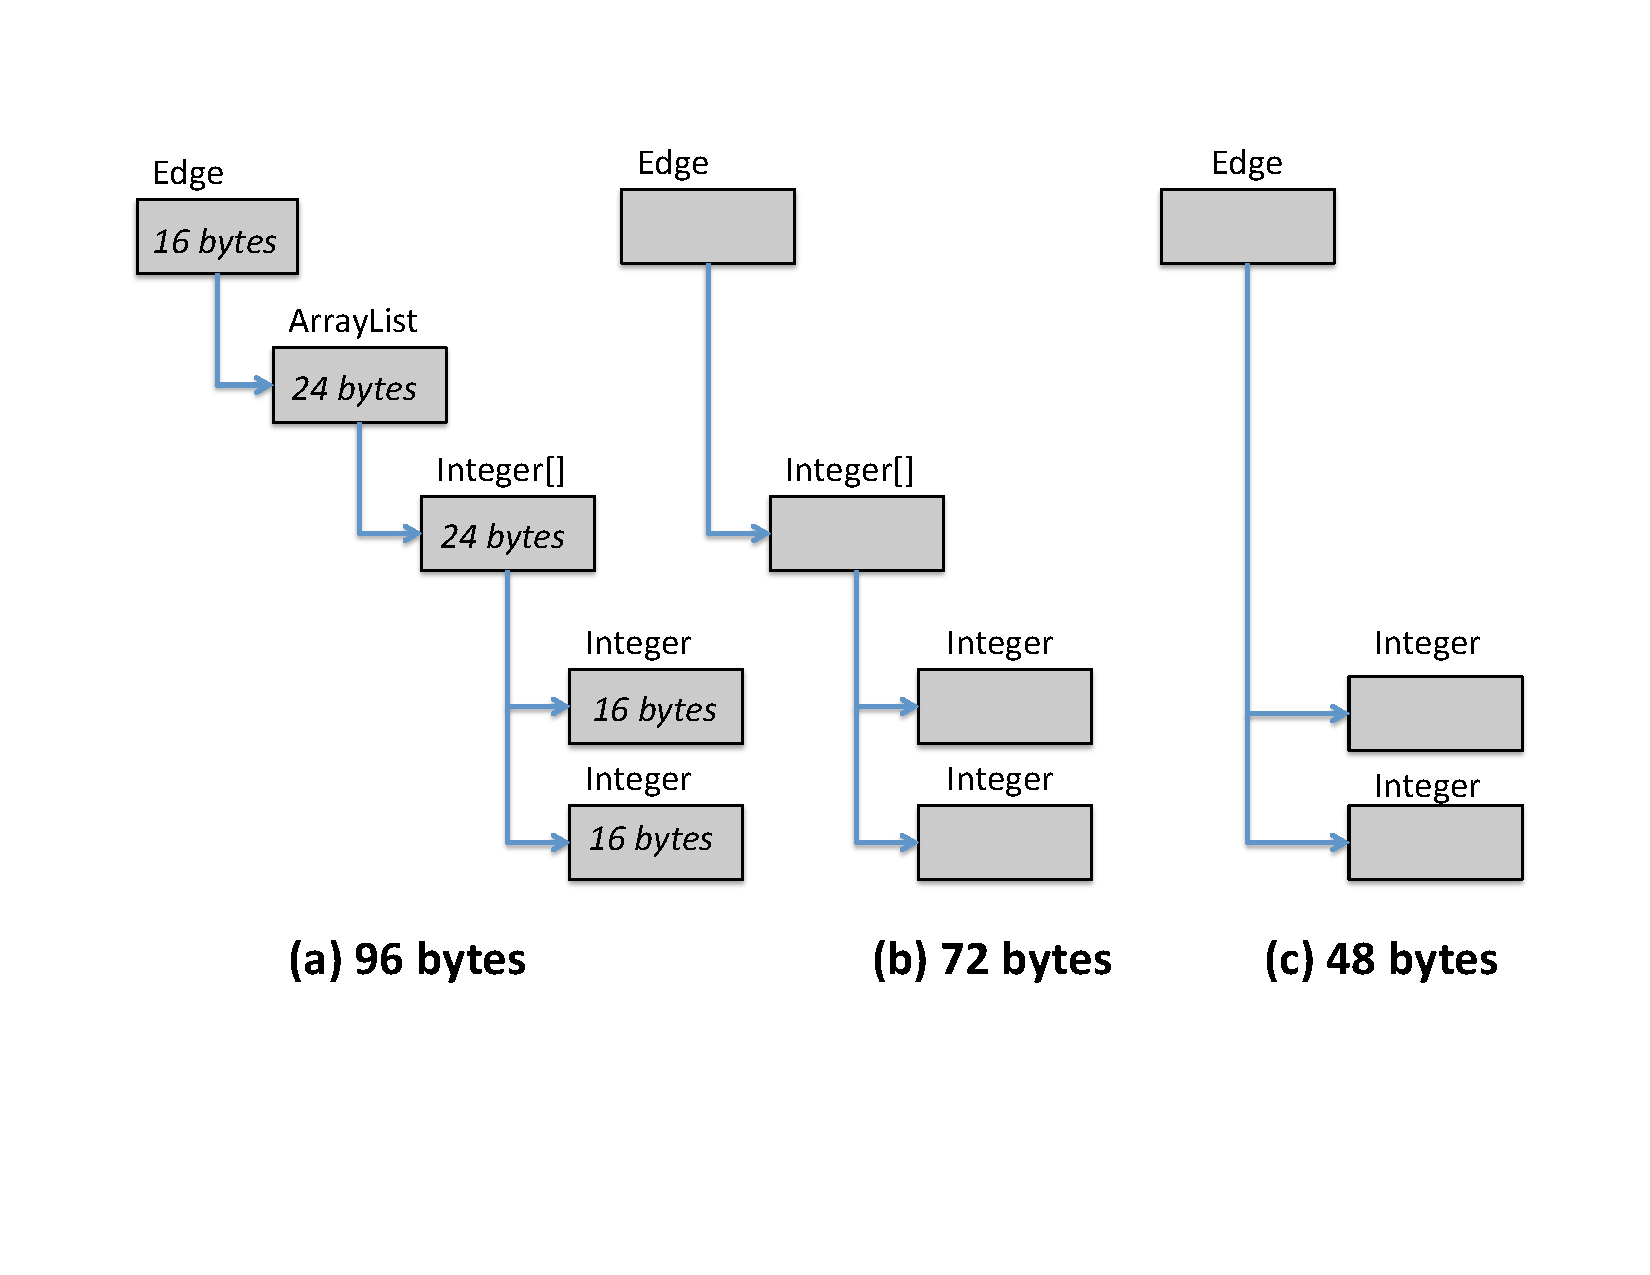
\includegraphics[width=.80\textwidth]{part1/Figures/collections/Edges.pdf}
%  \caption{(a) An \class{Edge} has 96 bytes. (b) Replacing the
%  \class{ArrayList} by an array eliminates 24 bytes. (c) Inlining the array
%  eliminates another 24 bytes.}
%  \label{fig:edges}
%\end{figure}
This is an example of choosing an overly-general collection. In
this situation, you don't need a collection at all. Using \class{ArrayList}
for storing fixed- or bounded-size arrays is a
common practice that can be easily avoided.

There is one final optimization that can be performed on the \class{Product}
class. Namely, making the four alternate suppliers into fields of
\class{Product} instead of elements of an array. This optimization
 a 32 byte array object for 75,000 products, while adding three additional
 fields to the \class{Product} for 100,000 objects, saving another 1.1MB in
 total:
\begin{shortlisting}
class Product {
	String sku;
	String name;
	.. 
	Supplier alternateSupplier1;
	Supplier alternateSupplier2;
	Supplier alternateSupplier3;
	Supplier alternateSupplier4;
}
\end{shortlisting}

This representation is very similiar to the original \class{Product} class in
section~\ref{sec:rarely-used} where there is one alternate suppler field, and
here there are four. Taking all of the optimizations 
together, we have gone from the initial \class{HashSet} representation
of 22.1MB in Section~\ref{section:choosing-collection} to the in-lined field
representation of 1.86MB. 

\section{Hybrid Representations}

An interesting case is when the sizes of the collections used in a relationship
is not uniform. That is, some collections are small and some collections are
very big.  It's reasonable to use an expensive collection like \class{HashSet}
for the big collections, but then the small collections pay the price. One way
to handle this problem is to use a hybrid representation. For example, you can
use arrays for smaller collections, and \class{HashSets} for larger
collections. 

One catch is that usually you will not know in advance which collections in the
relationship will end up being small and which will grow to be large. Therefore
a conversion operation will be necessary at some point if a collection grows
large enough. Each collection starts as an array, and then once it
grows past a threshhold, it is converted to a \class{HashSet}.

In our example, suppose that the vast majority of products have four alternate
suppliers on average, but a few products have over 100 alternate suppliers. We
can choose a threshhold, say six entries, which triggers a conversion to a
\class{HashSet} when the threshhold is exceeded. Here is the class
\class{Product}:

\begin{shortlisting} 
public class Product {

	    static final int threshhold = 6;
		String sku;
		String name;
		..
		int numAlternateSuppliers;
		Supplier[] alternateSuppliers;
		HashSet<Supplier> bigAlternateSuppliers;
		
		void addAlternateSupplier(Supplier supplier) {
		
		    /* Check for duplication */
		    if (hasAlternateSupplier(supplier)) {
		         return;
		    }
		
		    /* Try to add the supplier to the array alternateSuppliers */
		    if (numAlternateSuppliers == 0) {
		        alternateSuppliers = new Supplier[threshhold];
		    }
			if (numAlternateSuppliers < threshhold) {
			    alternateSuppliers[numAlternateSuppliers++] = supplier;
			    return;
			}
			
			/* If threshhold is exceeded, need to use bigAlternateSuppliers */
			if (numAlternateSuppliers == threshhold) {
			    bigAlternateSuppliers = new HashSet<Supplier>();
			    for (int i = 0; i < threshhold; i++) {
			    	bigAlternateSuppliers.add(alternateSuppliers[i]);
			    }
			    alternateSuppliers = null;
			}
			bigAlternateSuppliers.add(supplier);
			numAlternateSuppliers++;
			return;
		}
}
\end{shortlisting}
The method \code{addAlternateSupplier} adds the supplier to the array if the
size is less than the thresshold, otherwise, it adds the supplier to the \class{HashSet}.
It allocates the alternate supplier array and \class{HashSet} 
only if and when it is needed, to avoid wasting space with empty collections
when there are no or only a few alternate suppliers.

Implementing hybrid representations is more complicated than just using one
collection for a relationship. However, it can save significant space in some
cases.

\section{Summary}

Collections used to represent relationships often result in many small
collection instances, whose cost is dominated by a fixed-size
overhead. This chapter describes a number of ways to mitigate high fixed memory
costs for relationships implemented with collections:
\begin{itemize}
  \item Choose the most memory-efficient collection for the job at hand. In
  particular when collections have at most a few elements in them, you don't
  need expensive functionality like hashing. 
  \item Make sure collections are properly sized. If you know that a collection
  will not grow any more, then there is no reason to maintain extra room for
  growth.
  \item Avoid lots of empty collections. It is common to allocate collections 
 ahead of time, whether or not they will eventually ever be used. If you
 postpone creating them until they are needed, often you will end up with fewer collections, 
 and no empty collections.
 \item Use arrays instead of \class{ArrayLists} when you know the maximum size
 of the collections in advance. You can also eliminate an
 \class{ArrayList} altogether when there are always at most a few entries that
 can be stored in fields.
 \item When the usage pattern is not uniform, it is sometimes reasonable to use
 a hybrid representation.
\end{itemize}
Knowing which relationships and collections in your application are the most
important and need to scale is key to applying these optimizations effectively.  




